\section{SYSTEM DESIGN}

\subsection{ER-diagram}
ER-diagram is a high-level conceptual data model diagram. Entity
relation model is based on the notion of real-world entities and the
relationship between them. ER-diagram helps to explain the logical structures of
database. ER-diagrams are created depending on three basic concepts: entities,
attributes  and relationships. ER modelling helps you to analyse data
requirements systematically.

\vspace{1cm}
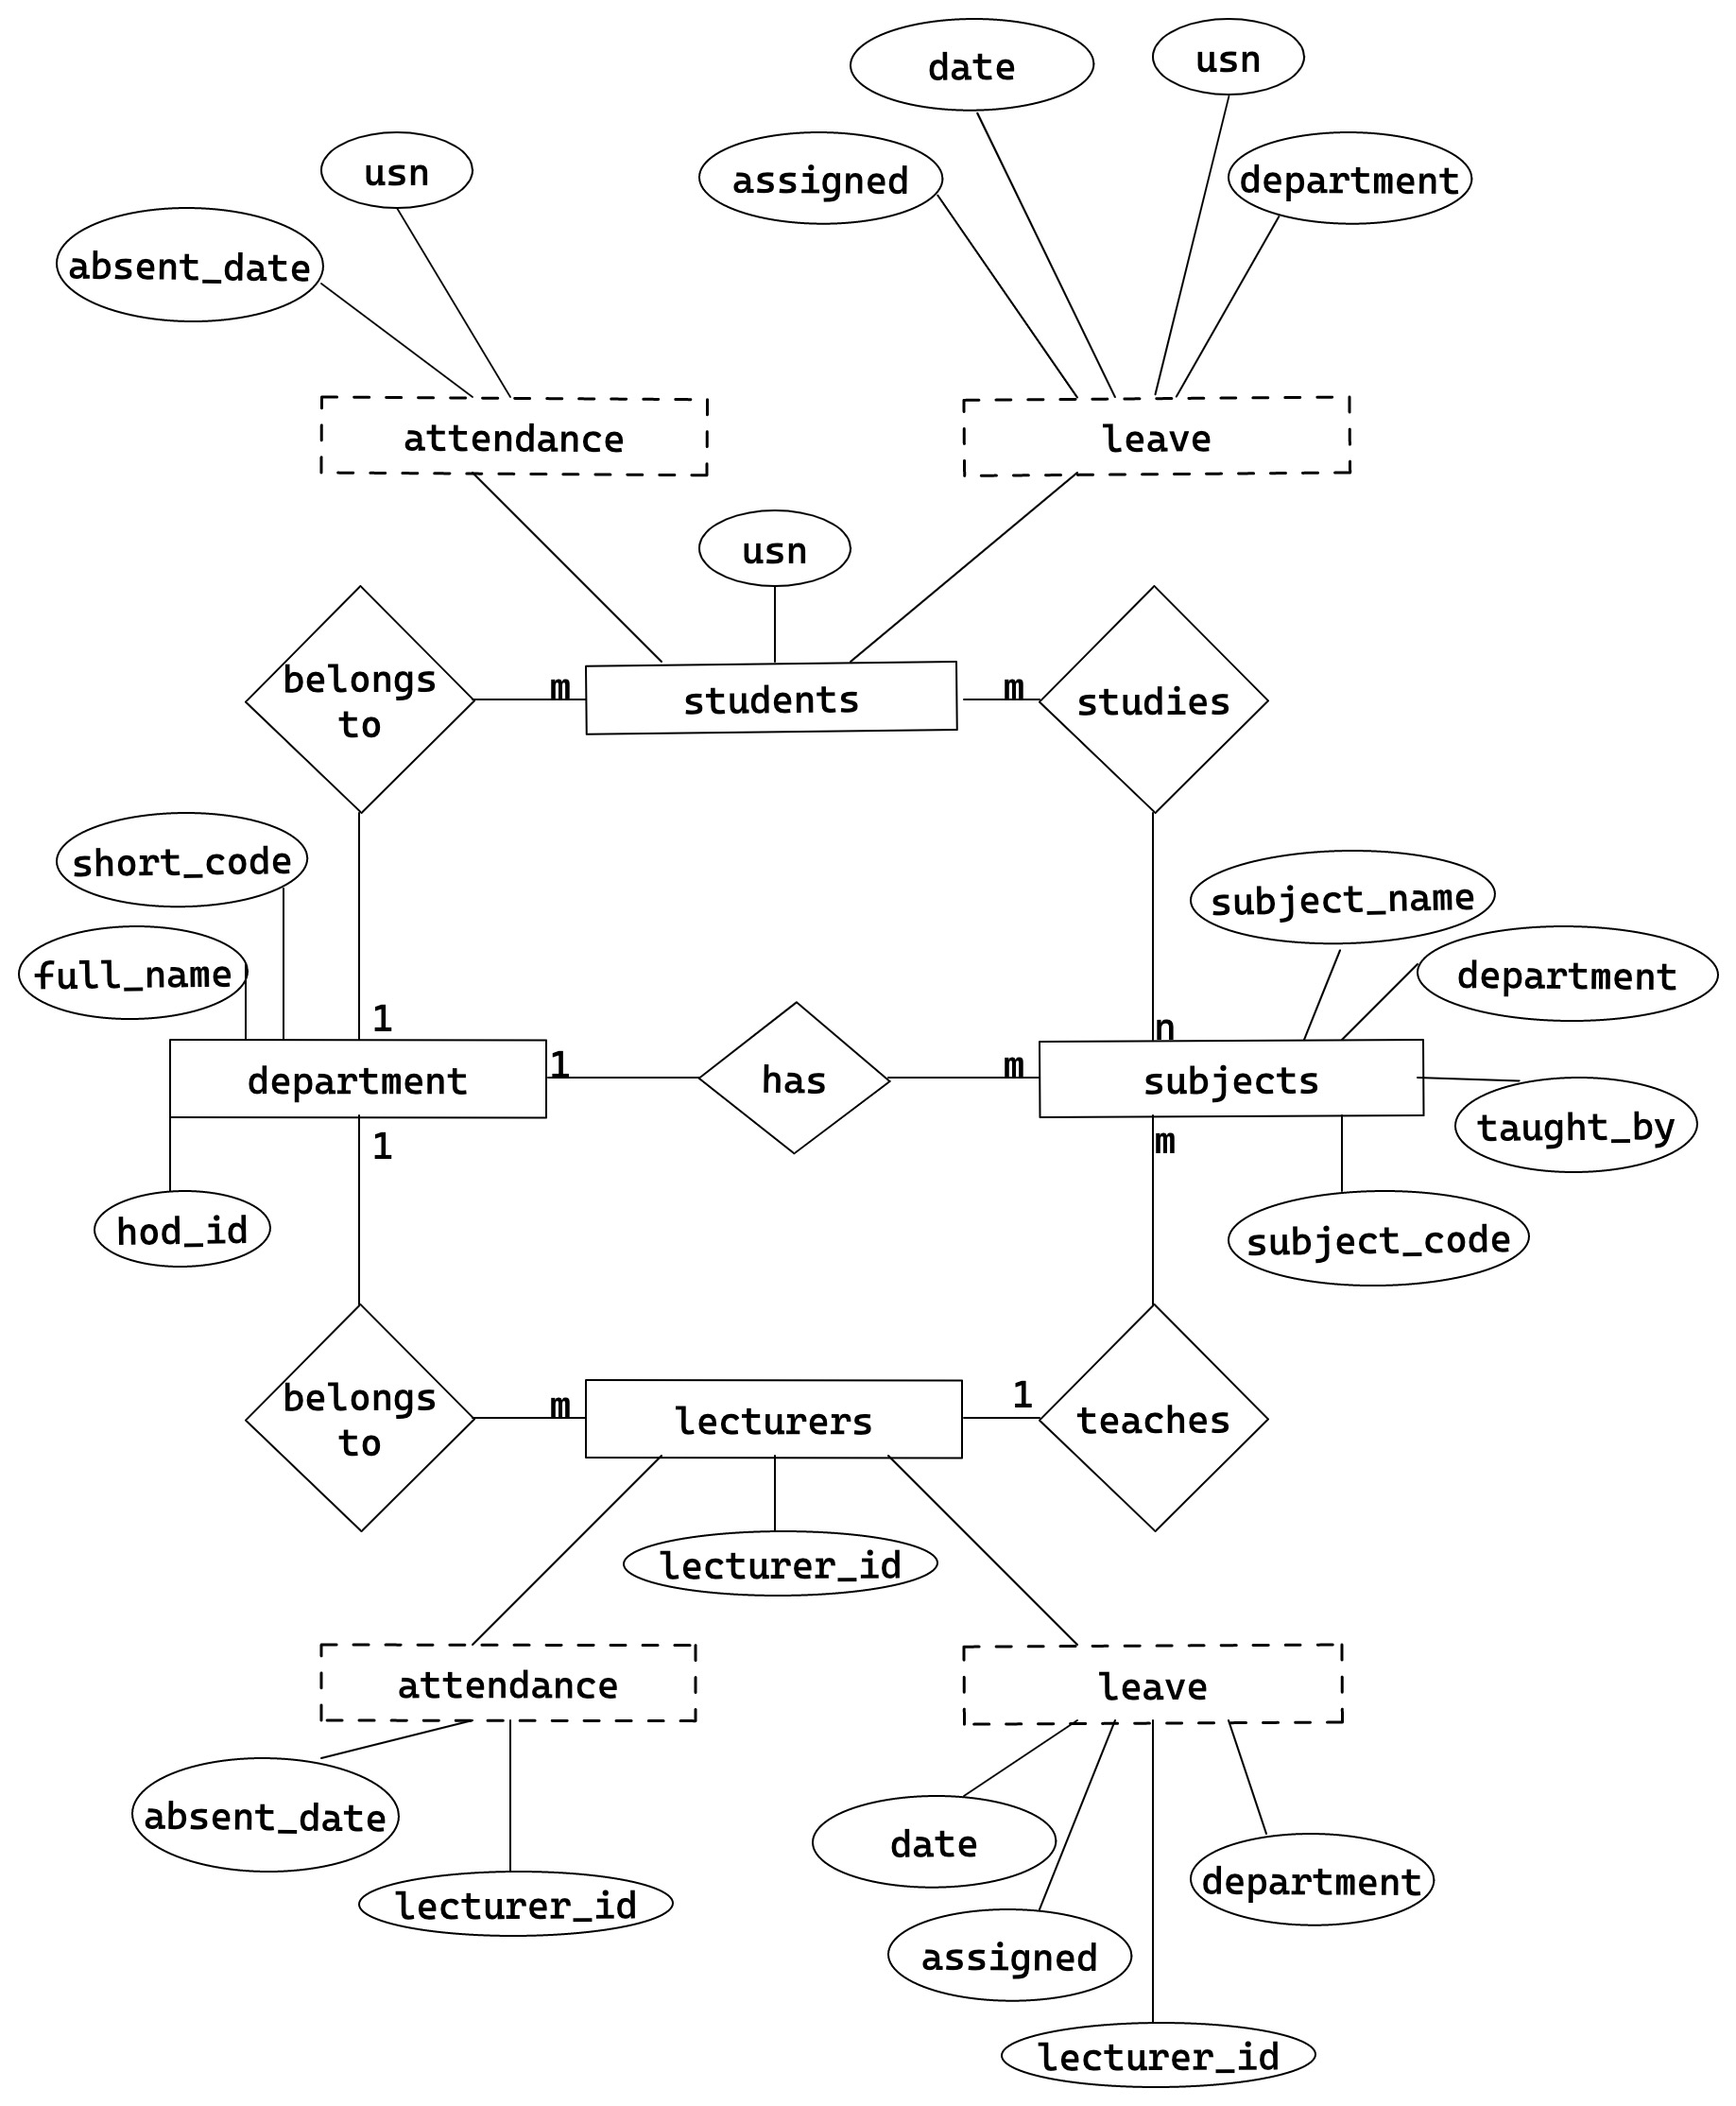
\includegraphics[width=14.5cm]{assets/er.jpeg}

\newpage
\subsection{Overview of Frontend}
The frontend of the proposed application is web-based, built using web
technologies like HTML, CSS, JavaScript. We choose to build web-based solution
so as to make it easily available to everyone without any friction. If we were
to build a PC native app or mobile native app then we would limit the
availability and so we decided to make a web-based application instead. We have
used ReactJS as our frontend framework which would enable us to reuse code, make
it easy to handle user data and states of application.

\subsubsection{About JavaScript}
JavaScript, often abbreviated as JS, is a programming language that is one of
the core technologies of the World Wide Web, alongside HTML and CSS. As of 2022,
98\% of websites use JavaScript on the client side for webpage behavior, often
incorporating third-party libraries. All major web browsers have a dedicated
JavaScript engine to execute the code on users' devices.

JavaScript is a high-level, often just-in-time compiled language that conforms
to the ECMAScript standard. It has dynamic typing, prototype-based
object orientation, and first-class functions. It is multi-paradigm, supporting
event-driven, functional, and imperative programming styles. It has application
programming interfaces (APIs) for working with text, dates, regular expressions,
standard data structures, and the Document Object Model (DOM).

\subsubsection{About ReactJS}
React is a free and open-source front-end JavaScript library for building user
interfaces based on UI components. It is maintained by Meta (formerly Facebook)
and a community of individual developers and companies. React can be used as a
base in the development of single-page, mobile, or server-rendered applications
with frameworks like Next.js. However, React is only concerned with state
management and rendering that state to the DOM, so creating React applications
usually requires the use of additional libraries for routing, as well as certain
client-side functionality

Some notable features of ReactJS are as follows:
\begin{enumerate}
    \item Declarative syntax
    \item Component based architecture
    \item Usage of Virtual DOM instead of directly modifying real DOM
    \item It uses JSX
    \item Management of state
    \item Updating only parts of the page according to state changes
\end{enumerate}

\subsection{Overview of Backend}
The backend is the part that connects to the database and manages the business
logic of the application, it isn't concerned with the UI but is mainly concerned
with how things work. We used NodeJS as the runtime for JavaScript so that we
can run our server application and wait for people to load the website. This
server is divided into multiple components or modules, one for authentication,
one for accessing data from the database.

\subsubsection{About NodeJS}
Node.js is a cross-platform, open-source server environment that can run on
Windows, Linux, Unix, MacOS, and more. Node.js is a back-end JavaScript runtime
environment, runs on the V8 JavaScript Engine, and executes JavaScript code
outside a web browser. As an asynchronous event-driven JavaScript runtime,
Node.js is designed to build scalable network applications

Node.js lets developers use JavaScript to write command line tools and for
server-side scripting. The functionality of running scripts server-side produces
dynamic web page content before the page is sent to the user's web browser.
Consequently, Node.js represents a "JavaScript everywhere" paradigm, unifying
web-application development around a single programming language, rather than
different languages for server-side and client-side scripts.

\subsubsection{About SQL}
Structured Query Language, abbreviated as SQL, is a domain-specific language
used in programming and designed for managing data held in a relational
database management system (RDBMS), or for stream processing in a relational
data stream management system (RDSMS). It is particularly useful in handling
structured data, i.e. data incorporating relations among entities and
variables.

Originally based upon relational algebra and tuple relational calculus, SQL
consists of many types of statements, which may be informally classed as
sublanguages, commonly: a data query language (DQL), a data definition
language (DDL), a data control language (DCL), and a data manipulation
language (DML). The scope of SQL includes data query, data manipulation
(insert, update, and delete), data definition (schema creation and
modification), and data access control. Although SQL is essentially a
declarative language (4GL), it also includes procedural elements.

SQL is the standard language for Relational Database System. All Relational
Database Management System (RDMS) like MySQL, Oracle, PostgreSQL, Microsoft SQL
Server use SQL as their standard database language.

\subsubsection{About PostgreSQL}
PostgreSQL, also known as Postgres, is a free, open-source, powerful, open
source object-relational database system that uses and extends the SQL language
combined with many features that safely store and scale the most complicated
data workloads

PostgreSQL features transactions with Atomicity, Consistency, Isolation,
Durability (ACID) properties, automatically updatable views, materialized views,
triggers, foreign keys, and stored procedures. It is designed to handle a range
of workloads, from single machines to data warehouses or Web services with many
concurrent users. It is the default database for MacOS Server and is also
available for Windows, Linux, FreeBSD, and OpenBSD.
